\documentclass[a4paper]{jpconf}
\usepackage{graphicx}
\begin{document}
\title{Use of glide-ins in CMS for production and analysis}
\author{D. Bradley$^1$, O. Gutsche$^2$, K. Hahn$^3$, B. Holzman$^2$, S. Padhi$^{4,}$\footnote[6]{corresponding author, email: sanjay.padhi@cern.ch}, H. Pi$^4$, D. Spiga$^5$, I. Sfiligoi$^2$, E. Vandering$^2$, F. W\"urthwein$^4$}
\address{$^1$ University of Wisconsin-Madison, Madison, WI, USA}
\address{$^2$ Fermilab, Batavia, IL, USA}
\address{$^3$ Massachusetts Institute of Technology, Cambridge, MA, USA}
\address{$^4$ University of California, San Diego, La Jolla, CA, USA}
\address{$^5$ CERN, CH-1211 Geneva, Switzerland}
%%%%%%%%%%%%%%%%%%%%%%%%%%%%%%%%%%%%%%%%%%%
\author{(On behalf of the CMS Offline and Computing Projects)}
%%%%%%%%%%%%%%%%%%%%%%%%%%%%%%%%%%%%%%%%%%%
\begin{abstract}
%%%%%%%%%%%%%%%%%%%%%%%%%%%%%%%%%%%%%%%%%%%
With the evolution of various grid federations, the Condor glide-ins represent a key feature in providing a homogeneous pool of resources using late-binding technology. The CMS collaboration uses the glide-in based Workload Management System, glideinWMS, for production (ProdAgent) and distributed analysis (CRAB) of the data. The Condor glide-in daemons traverse to the worker nodes, submitted via Condor-G. Once activated, they preserve the Master-Worker relationships, with the worker first validating the execution environment on the worker node before pulling the jobs sequentially until the expiry of their lifetimes. The combination of late-binding and validation significantly reduces the overall failure rate visible to CMS physicists. We discuss the extensive use of the glideinWMS since the computing challenge, CCRC-08, in order to prepare for the forthcoming LHC data-taking period. The key features essential to the success of large-scale production and analysis at CMS resources across major grid federations, including EGEE, OSG and NorduGrid are outlined. Use of glide-ins via the CRAB server mechanism and ProdAgent, as well as first hand experience of using the next generation CREAM computing element within the CMS framework is discussed.
\end{abstract}
%%%%%%%%%%%%%%%%%%%%%%%%%%%%%%%%%%%%%%%%%%%
\section{Introduction}
%%%%%%%%%%%%%%%%%%%%%%%%%%%%%%%%%%%%%%%%%%%
The CMS collaboration has adopted Grid computing as its base computing model to simplify the deployment and management of the
tens of thousand of CPUs needed to accomplish its mission.
While the Grid computing paradigm has proven to be a boon for resource providers, 
allowing them to keep their administrative autonomy over the resources they manage,
the added abstraction layer has introduced several problems for the users, 
ranging from higher complexity to decreased reliability.

One solution that has proven to significantly reduce user problems is the late-binding, or pilot technology.  
A late-binding Workload Management System (WMS) hides the complexity of the Grid environment by dynamically creating 
a virtual private pool of compute resources, thus giving users an environment similar to a dedicated batch cluster.
This paper describes the experience of the CMS collaboration with one late-binding WMS implementation called glideinWMS. 
%%%%%%%%%%%%%%%%%%%%%%%%%%%%%%%%%%%%%%%%%%%
\section{Late binding based Workload Management System - GlideinWMS }
%%%%%%%%%%%%%%%%%%%%%%%%%%%%%%%%%%%%%%%%%%%
The Grid paradigm calls for the compute resources to be partitioned into multiple independent pools, called Grid sites,
with only a thin common layer to provide interoperability, as shown in Fig.~\ref{fig:glideinWMS}.
Without some additional tools, this approach makes the life of a Grid user quite unpleasant. 

The four major problems the users experience are:
\begin {itemize}
\item 
A user must partition his/her jobs between the resource pools.
Finding the optimal partition is far from an easy task, as explained below.
\item
At any Grid site, the common layer provides only very limited information about the status and policies of the
batch system that handles the local resource pool.
This is a necessary evil that allows the common layer to present the information from all the different batch system 
implementations in a uniform way. 
\item 
The common layer provides only very limited information about the progress of a job, once it is accepted at a Grid site.
Again, this is a necessary evil that allows the common layer to monitor jobs submitted to different batch systems.  
\item
Each Grid site is allowed to configure the worker nodes the way it likes, within very permissive limits.
Users are expected to write their compute jobs in such a way to automatically adapt to any condition they encounter.
\end{itemize}
\begin{figure}
\begin{center}
\includegraphics[scale=0.5]{glideinWMS_arch}
\end{center}
\caption{Overview of glideinWMS system.}
\label{fig:glideinWMS}
\end{figure}

The approach taken by the late binding Workload Management Systems (WMS) to ease the user burden is 
to create a dynamic virtual private pool of compute resources by submitting pilot jobs to the Grid sites.
Once a pilot job starts, it joins the virtual private pool and starts a user job from the late binding WMS job queue, 
as shown in Fig.~\ref{fig:glideinWMS}.

This insulates the users from the Grid layer, giving users
the impression of running on a single, local, dedicated pool of compute resources
and thus eliminating, or at least reducing the magnitude of the above mentioned major problems:
\begin {itemize}
\item 
By having a single resource pool, no job partitioning is needed.
\item
Detailed information about the status and policies of the virtual private pool can be made available, 
since users can use the tools provided by the specific implementation of the late binding WMS instance used.
\item 
Detailed information about the progress of a job can be made available,
since users can use the tools provided by the specific implementation of the used late binding WMS instance.
\item
The late binding WMS can reduce the heterogeneity of the compute resources, 
by either only gathering properly configured worker nodes,
or by providing wrapper scripts that provide common tools and libraries.
\end{itemize}

The late binding WMS used by CMS is called \textbf{glideinWMS}. GlideinWMS is based on the Condor batch system, 
with the addition of a thin layer responsible for the submission of the pilot jobs.

A glideinWMS virtual private pool consists of a regular Condor pool, 
where worker node Condor daemons, i.e. \emph{condor\_startd} and \emph{condor\_starter}, 
have been downloaded, configured and started by a glideinWMS pilot job; such pilot jobs are known as \emph{glide-ins}. 
Since the different Condor daemons are dispersed around the world and use wide area networking to communicate to each other,
the daemons are configured to use strong, X.509 based authentication for authorization and message integrity purposes.
The worker node Condor daemons are also configured to have a limited lifetime, in order to fit within the wall-clock limits 
of the batch system of the Grid site they are running on.
For all other practical purposes, the resulting Condor pool is indistinguishable from a dedicated Condor pool without a shared file system.

The submission of glide-ins is regulated by two types of daemon processes; 
one or more \textbf{glide-in factories} and one or more \textbf{VO frontends}. 
The two types of processes communicate by means of ClassAds using a dedicated \emph{condor\_collector} daemon:
\begin{enumerate}
\item A glide-in factory advertises what Grid sites it knows about, and can submit to, together with the characteristics of the site 
(for example: what versions of CMS software are installed there).
\item The VO frontend queries the user queues, i.e. the \emph{condor\_schedds}, 
matches the found jobs with the factory ClassAds, 
and then advertises how fast the factory should submit new glide-ins.
\item Finally, the factory reads the VO frontend ClassAds and starts submitting the glide-ins at the specified rate.
\end{enumerate}

All together make the system work as illustrated in Fig.~\ref{fig:glideinWMS}.
\begin{figure}
\begin{center}
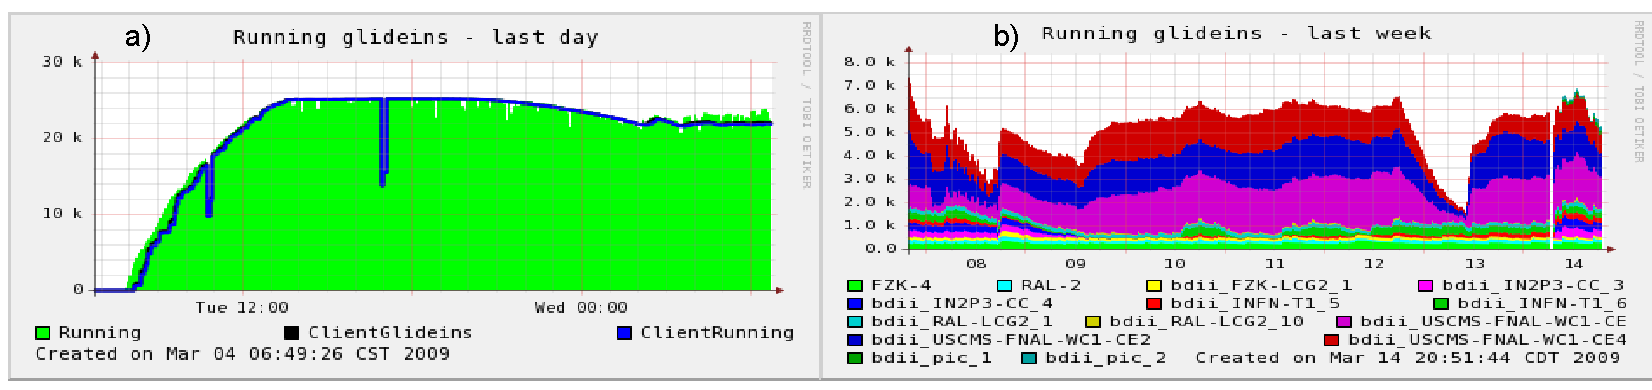
\includegraphics[scale=0.55]{glideinT1stat}
\end{center}
\caption{Number of simultaneous running glide-ins for: a) scalability studies and b) CMS data re-processing at Tier-1 centers.}
\label{fig:glideinT1stat}
\end{figure}
%%%%%%%%%%%%%%%%%%%%%%%%%%%%%%%%%%%%%%%%%%%%%%%%%%%%%%%%%%%%%%%%
\subsection {Interoperability between EGEE, OSG, and NorduGrid}
%%%%%%%%%%%%%%%%%%%%%%%%%%%%%%%%%%%%%%%%%%%%%%%%%%%%%%%%%%%%%%%%
In principle, the problem of interoperability between different grids is reduced to having a Condor-G client
for submission of the glide-ins for the particular grid flavor. All other incompatibilities can be 
resolved via appropriate configuration of the glide-ins. In practice, CMS deals with many of the differences 
between EGEE and OSG inside the CRAB or ProdAgent layers of the software stack, thus requiring little special 
configuration in the glide-ins. As part of our work for the Common Computing Readiness Challenge 08 (CCRC-08), we worked 
with the Condor team on the details of submitting glide-ins via Condor-G to grids such as the NorduGrid. The method 
consists of using protocol-specific modules called GAHPs (Grid Ascii Helper Programs) along with logics in the Condor gridmanager for the 
specific use of it, when submitting to a given grid flavor. This resulted 
in the first ever use of NorduGrid resources for data analysis within CRAB using glideinWMS. The other grid flavors like 
EGEE and OSG CEs are accessible using gt2 protocols via the Condor-G client. This developments led to
a fully interoperable system across various grid flavors for the first time.
\begin{figure}
\begin{center}
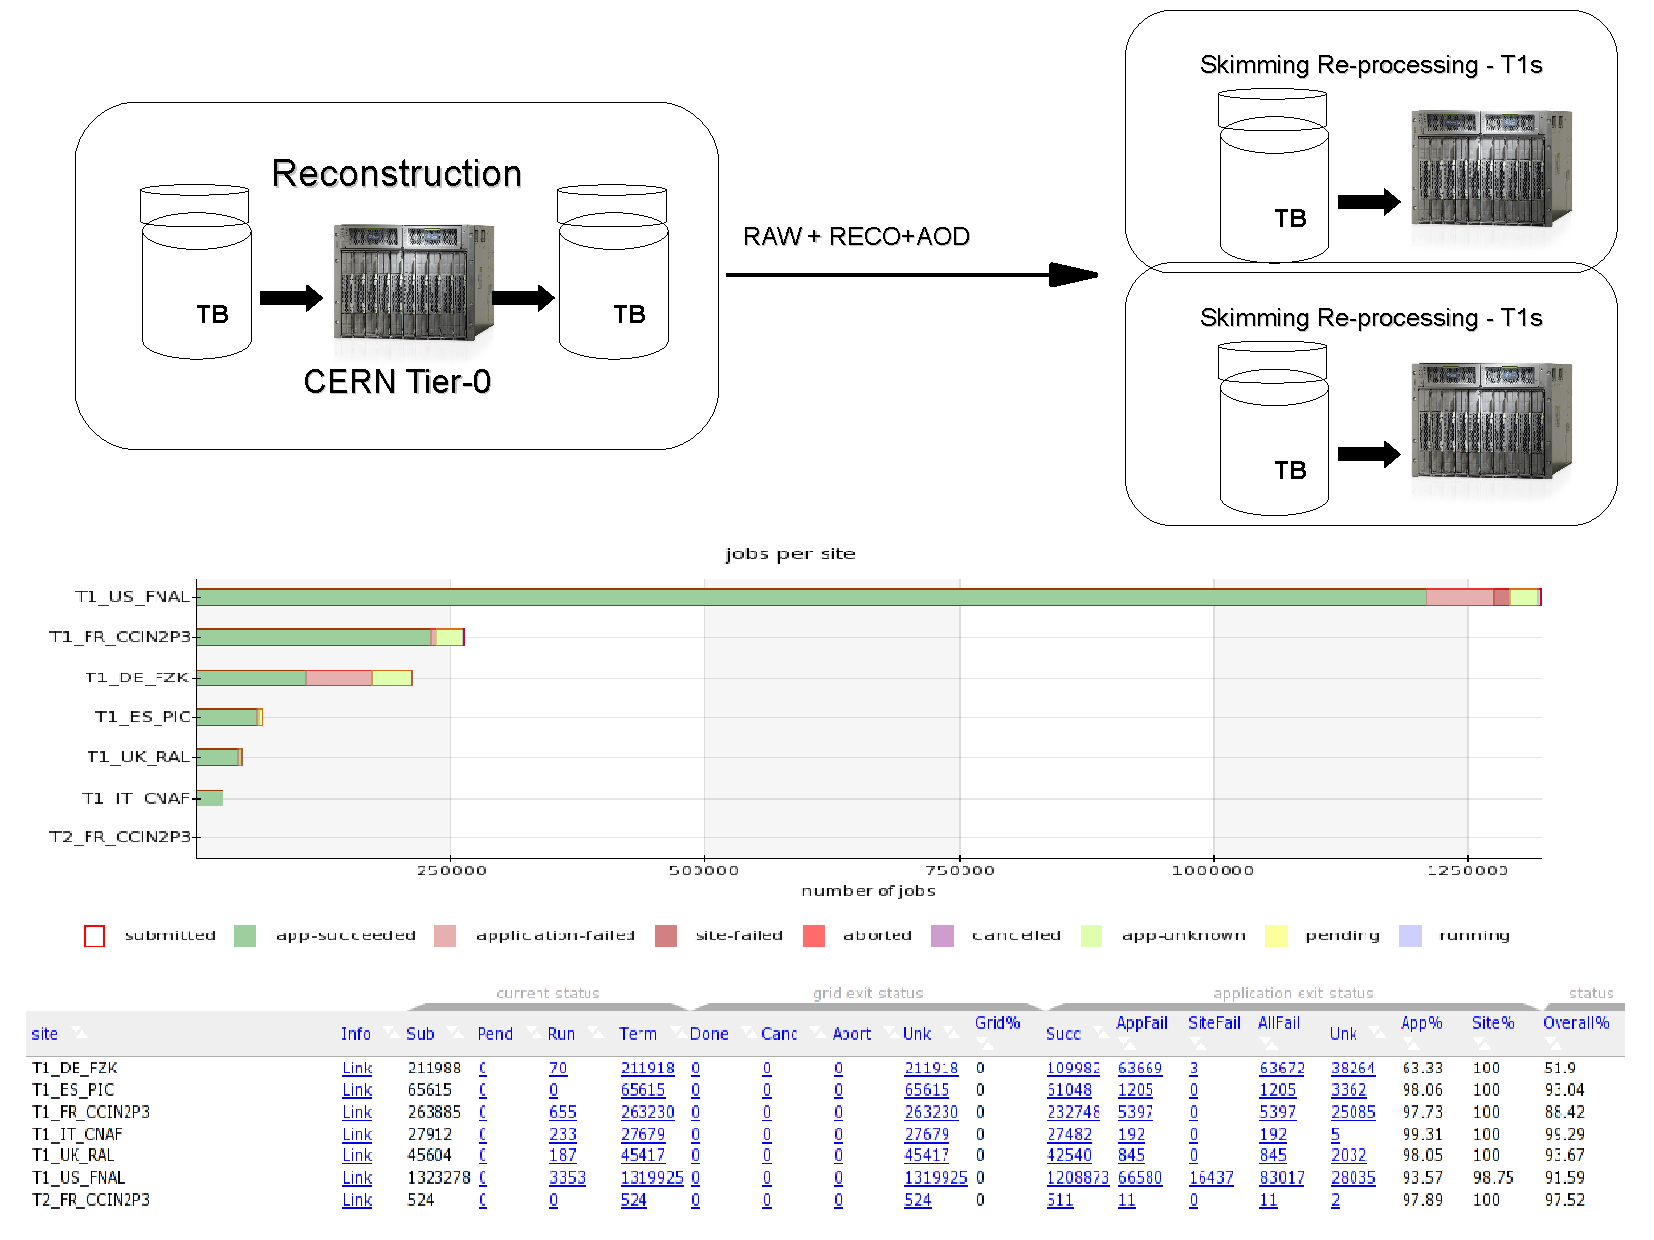
\includegraphics[scale=0.5]{DataReprocess}
\end{center}
\caption{Overview of CMS data re-processing and resource usage statistics using glideinWMS.}
\label{fig:reprocessT1s}
\end{figure}
%%%%%%%%%%%%%%%%%%%%%%%%%%%%%%%%%%%%%%%%%%%%%%%%%%%%%%%%%%
\subsection {Scalability of the system}
%%%%%%%%%%%%%%%%%%%%%%%%%%%%%%%%%%%%%%%%%%%%%%%%%%%%%%%%%%
The scalability of the system has been intensively tested over the WAN, especially over large distances such 
as between US and Europe. Various components were identified which could have an effect on
latencies in communications between the glide-in \emph{startds} and the central managers. Many improvements were
made both in reducing the cost of authentication, as well as enhancing the speed in matchmaking and 
the security sessions. The details of the study can be found in \cite{bib:scalability}. The overall improvement 
from this study lead to the simultaneous running of jobs between 23k to 25k as shown in Fig.~\ref{fig:glideinT1stat}a).
More than 500k jobs were submitted with an average running period of 3 hours. The successful usage
of the Two-Tier Collector model using a single 1.5GHz Pentium 4 machine, capable of harnessing more than 25k 
resources gives us the confidence of using the system for collaboration-wide data analysis and monte carlo 
productions.
%%%%%%%%%%%%%%%%%%%%%%%%%%%%%%%%%%%%%%%%%%%%%%%%%%%%%%%%%%%%%%%%%%%%%%%%%%%%%%
\section{Use of glideinWMS for Production and Data Reprocessing }
%%%%%%%%%%%%%%%%%%%%%%%%%%%%%%%%%%%%%%%%%%%%%%%%%%%%%%%%%%%%%%%%%%%%%%%%%%%%%%
The CMS computing architecture \cite{bib:cms_computing_arch} is based on a tier-organized structure of computing
resources, based on a Tier-0 center at CERN and 7 Tier-1 centers for organized mass data processing. 
The Tier-0 is in charge of storing the data coming from the detector onto mass storage, performing a prompt 
reconstruction of the data and distributing the data among the Tier-1 centers. The Tier-1 sites archive on
mass storage their share of data, run data reprocessing, organized group physics analysis for data
selection and distribute the selected data to Tier-2s for user analysis. Tier-1 centers also
have the responsibility of storing Monte Carlo (MC) data produced at the Tier-2 sites. 

Fig.~\ref{fig:reprocessT1s} depicts the dataflows, workflows and computing resources involving the Tier1 sites.
The workflows and dataflows are conducted using glideinWMS  as well as CMS-specific services 
built on top of them. Data transfers are managed by the CMS data transfer and placement 
system PhEDEx \cite{bib:cms_phedex}. Tier-1s receive from CERN a continuous data stream of reconstructed data, data skimming 
is then conducted at the Tier-1 sites. Skimming jobs are run on a number of filters producing the 
corresponding output files with the selected events. ProdAgent is used to carry out the skimming workflow. 
It automatically prepares the skimming jobs for the sample to be filtered, submits to the glideinWMS and finally
launches the corresponding merge jobs. More than 1.9 million jobs were successfully processed at various 
Tier-1s, with a remarkable efficiency of approximately 96\% within last 3 months, using glideinWMS as shown 
in Fig.~\ref{fig:reprocessT1s}
\begin{figure}
\begin{center}
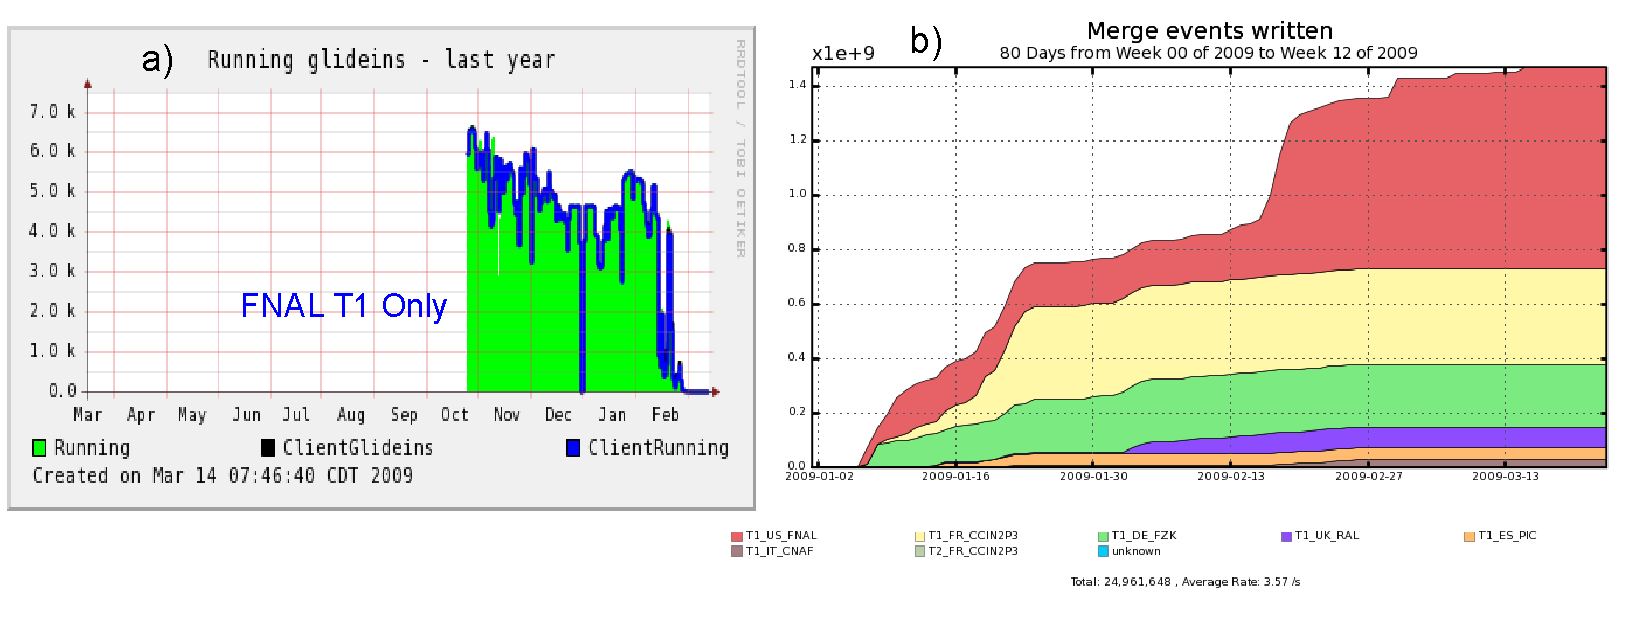
\includegraphics[scale=0.55]{merged_events}
\end{center}
\caption{a) Number of simultaneous running glide-ins at Fermilab during Oct.08 - Feb.09. b) Distribution of 
events merged as a function of time, written at various CMS Tier-1 centers.}
\label{fig:merged_events}
\end{figure}
Fig.~\ref{fig:glideinT1stat}b) shows the number of simultaneous glide-ins running at various Tier-1 centers during the last week of Mar.09. 
More than 1400 million events as shown in Fig.~\ref{fig:merged_events}b) are reprocessed and merged in last 80 days, which are then 
used for physics analyses at the Tier-2 centers. 

One of the essential features of the glideinWMS is the capability to utilize a large number of
resources, within very short fraction of time. As discussed earlier, most of the reprocessing task 
workflows involve numerous amounts of short jobs. Previous studies have shown that a given CE can 
afford a rate of \~0.1Hz number of jobs. In order to fill 6k resources at this rate, it would normally take 
about 16.67 hours.  The glide-in approach, however allows the workers (\emph{startds}) with ``long'' lived proxies. 
Each of these \emph{startds} can pull the client jobs in parallel and can sequentially process them until 
the expiry of their lifetimes. This provides a scalable solution for Tier-1 centers such as Fermilab, 
where a large number of resources are required to be used efficiently, which otherwise would not 
be possible to harness the effectively using traditional early-binding approach.
%%%%%%%%%%%%%%%%%%%%%%%%%%%%%%%%%%%%%%%%%%%%%%
\section{Use of glideinWMS for data analysis}
%%%%%%%%%%%%%%%%%%%%%%%%%%%%%%%%%%%%%%%%%%%%%%
\begin{figure}
\begin{center}
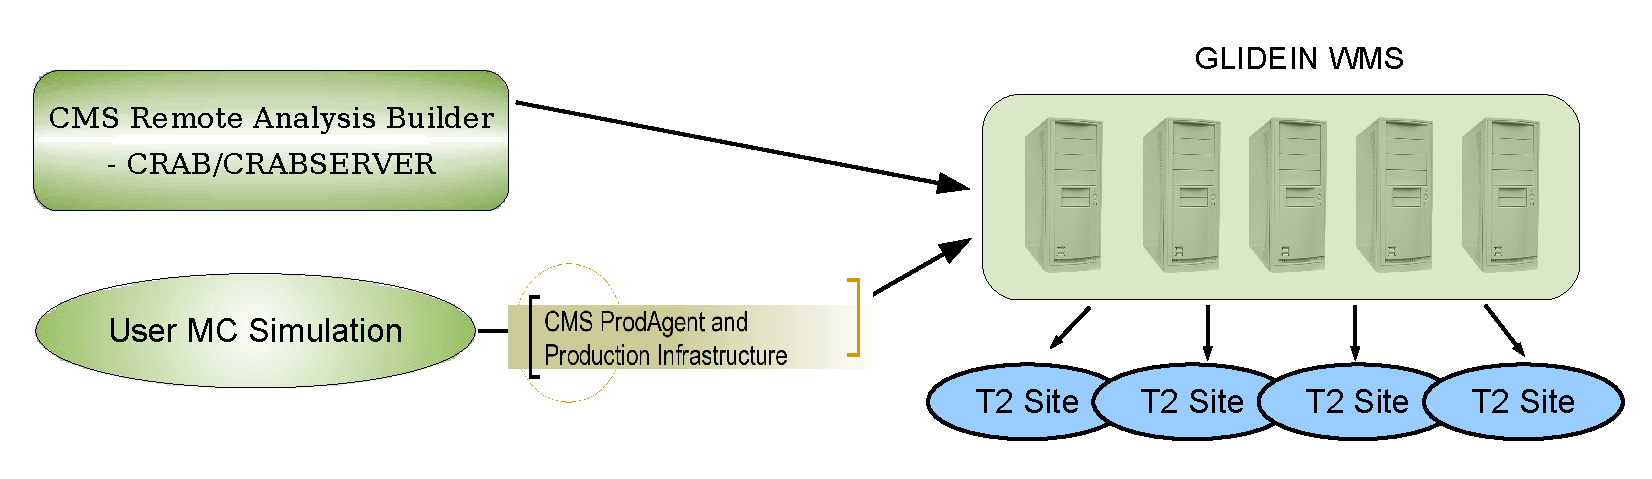
\includegraphics[scale=0.4]{user_analysis}
\end{center}
\caption{Schematic diagram of glideinWMS associated with user analyses activities.}
\label{fig:user_analysis}
\end{figure}
The data analysis on a distributed environment is a complex computing task. The CMS Collaboration
uses CRAB \cite{bib:cms_crab}, either via client or server in order to perform user analyses at the Tier-2 centers.
CRAB is a CMS specific software layer build on top of a WMS, such as glideinWMS. It simplifies the process 
of data analysis, job submission and retrieval by hiding much of the possible grid complexity from the
end user. The tool splits the analysis task into several jobs based on the requested number of events and
the location of input dataset via Dataset Bookkeeping System (DBS). Furthermore, it performs various checks along with 
packaging of the executables/libraries before submitting the jobs to the glideinWMS. The glideinWMS based 
on a tag of \emph{``DESRIED\_GATEKEEPER''} submits pilots/glide-ins to the requested site. Once the glide-ins are activated, 
it pulls the ``real'' user job from the queue after the matchmaking. During the process of activation, the 
initially submitted glide-ins perform various checks at the Worker Nodes (WN), such as the presence of the desired 
CMS software. Periodic updates are performed about the status of the job via glideinWMS to CRAB. Once the 
job is completed, the WMS provides the log files (stdout/stderr). The overall process also includes updates 
to the CMS Dashboard via Monalisa as the transport agent, for user jobs.
%%%%%%%%%%%%%%%%%%%%%%%%%%%%%%%%%%%%%%%%%%%
\subsection{CMS User Analysis and CCRC-08}
%%%%%%%%%%%%%%%%%%%%%%%%%%%%%%%%%%%%%%%%%%%
\begin{figure}
\begin{center}
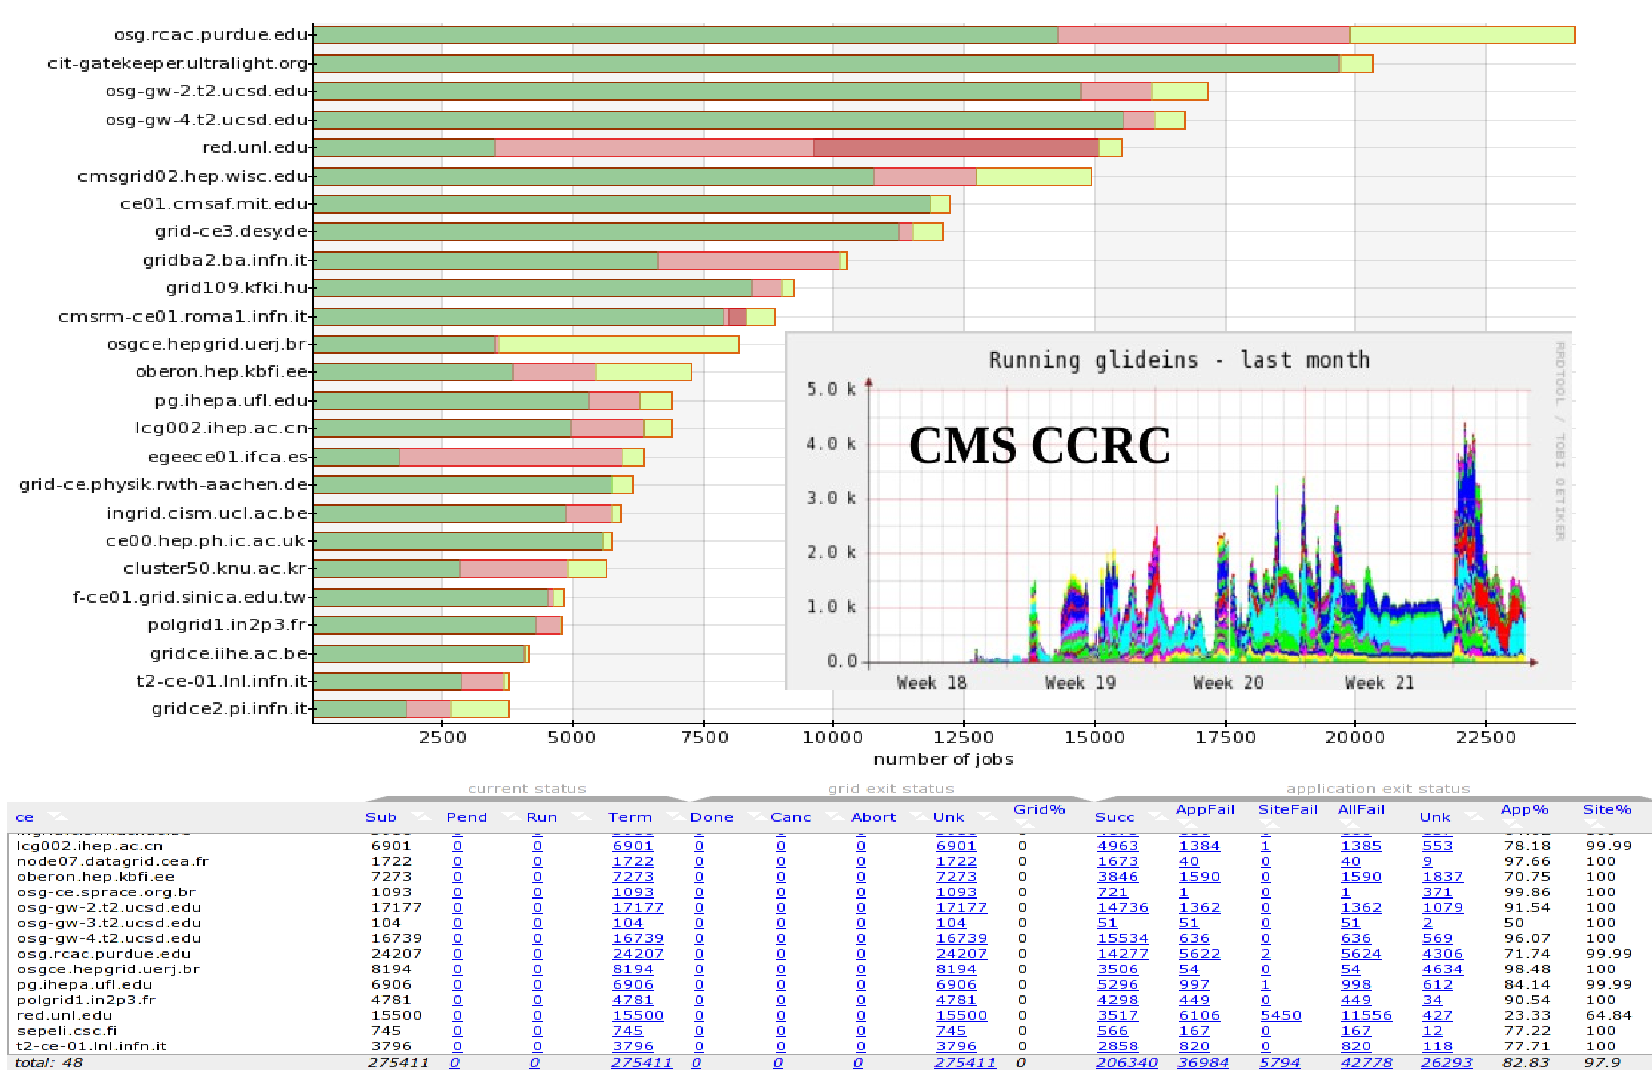
\includegraphics[scale=0.55]{glideins_ccrc08}
\end{center}
\caption{Usage of glideinWMS during CCRC-08 exercise.}
\label{fig:glideins_ccrc}
\end{figure}
The glideinWMS was intensively used during the CCRC-08. The goal was to gain an overall understanding 
of the performance and readiness of the CMS Tier-2 sites for data analysis. The input datasets needed for CCRC-08 were transferred
via the PhEDEx. Centrally organized workflows were used for this activity. The site performance
was evaluated using different types of jobs based on increasing complexity. The long-running 
CPU intensive jobs with moderate I/O, were aimed at understanding the site performance without
heavy loads on the storage systems. The short-running jobs with local stage out were targeted
to evaluate the performance of the site storage elements (SE). Intensive I/O with remote stage out
jobs were used not only to mimic the scenario of a real user performing data analyses, but also
to understand the site access to the back-end storage.

Over 40 sites across EGEE, OSG and Nordugrid were involved during this exercise. NorduGrid sites 
were harnessed for the first time in CMS. Fig.~\ref{fig:glideins_ccrc} shows overall results recorded in the CMS dashboard 
during the month long exercise. There were a mix of errors at a few sites due to catastrophic storage 
failures. The overall success rate, without SE issues ranged from 92-99\%, based on more than 200k 
submitted jobs using glideinWMS. The gliteWMS was also used during this exercise \cite{bib:cms_glite}.
%%%%%%%%%%%%%%%%%%%%%%%%%%%%%%%%%%%%%%%%%%%
\subsection{Studies using Crabserver and JobRobots}
%%%%%%%%%%%%%%%%%%%%%%%%%%%%%%%%%%%%%%%%%%%
Crabserver is a novel approach towards decoupling the user activities with the stack of software
layers responsible for performing the actual workload. The user submission is a simple layer 
of job submission and retrieval using CRAB client. On the other hand, the Crabserver is expected 
to have a nucleus of expertize, aggregated at a given site hosting the aforesaid server. User jobs
are submitted using the information from the DBS, as well as their credentials.
These are sent to the server using grid-ftp. Crabserver consists of several daemons that are responsible 
for Jobtracking, Tasktracking, Task lifetime managers, Command managers, etc. These processes
essentially ensure all the (re)submission/retrieval activities of a given task are correctly communicated
to the WMS, in this case glideinWMS. The glideinWMS then submits them to respective sites 
by preserving the user identity, as well as privileges via GUMS and glexec. The user credentials
and priorities are maintained by the WMS using Condor.

The University of California, San Diego (UCSD) is one of the centers responsible for hosting 
the Crabserver using glideinWMS for CMS user analyses. UCSD maintains a developmental as well 
as a production server both of which uses glide-in based WMS. The crabserver was tested to a very large 
scale using so-called ``JobRobots''. The JobRobots consist of a collection of agents, each 
managing a specific aspect of the job management (creation, submission, status
update, output collection). At regular time intervals, it creates for
each site a new analysis task to be run on a specific dataset. The
task is split into several jobs, that are submitted as a collection to
the Crabserver, which eventually submits to glideinWMS. Each job
performs a trivial data analysis on a fraction of the dataset, and when
finished, its output is retrieved. All submitted jobs are classified
as successful, failed at the application level or aborted at the Grid
level.
\begin{figure}
\begin{center}
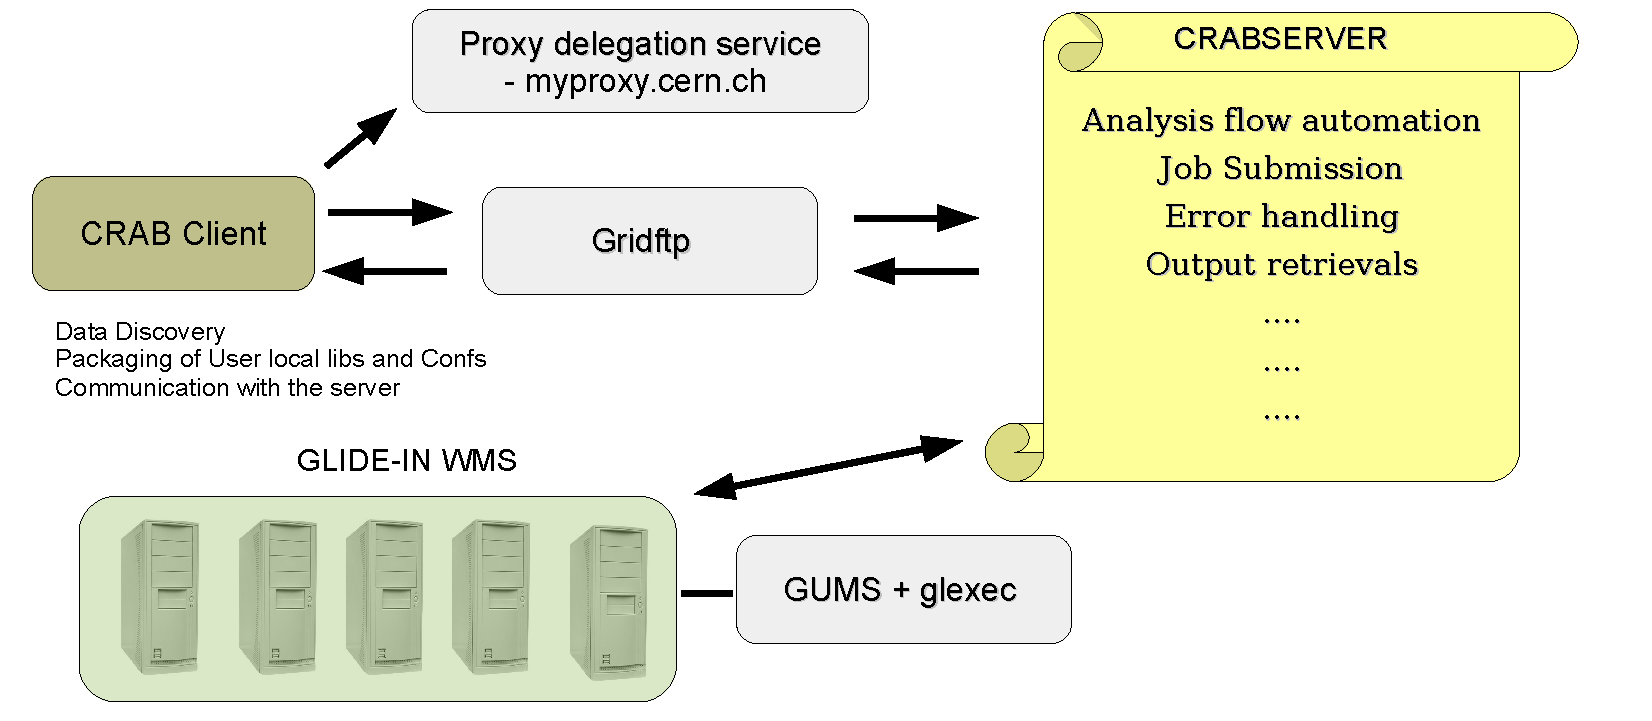
\includegraphics[scale=0.4]{crabserver}
\end{center}
\caption{Schematic diagram of Crabserver in association with glideinWMS.}
\label{fig:crabserver}
\end{figure}
The JobRobot daily statistics are not only used to measure the success rate for each site, 
but also to evaluate the Crabserver performance at UCSD, before the server can be allowed 
to be accessed by the general users. More than 25k jobs were submitted within a span of a 
few days, using JobRobots to the Crabserver. Several issues related to monitoring, 
submission/retrieval, delays, etc. were identified and fixed during this study. Various scalability
related issues are currently under study and are expected to be fixed in the forthcoming
release version of the server.
%%%%%%%%%%%%%%%%%%%%%%%%%%%%%%%%%%%%%%%%%%%
\subsection{User level MC production using Crabserver}
%%%%%%%%%%%%%%%%%%%%%%%%%%%%%%%%%%%%%%%%%%%
In CMS the MC production is performed using centrally a organized mechanism. However,
for small scale understanding of a given origin of physics model, it becomes too cumbersome
to involve the management resources. Thus, it is essential to have a simple interface
in order for the users to be involved in small scale MC productions. 

A http frontend is used to send production configuration to the system. 
The system uses X.509 authentication and authorization and also maintains the user priorities. 
It then creates the production workflow. The task is split into jobs via ProdAgent and then 
submitted to the glideinWMS as illustrated in Fig.~\ref{fig:user_analysis} It inherits the monitoring of the 
jobs via ProdAgent and glideinWMS tools. 
Once the jobs are completed it publishes the output into the local DBS instance. The registered 
dataset in the local DBS can be used by any member from the collaboration, like any other dataset produced 
by the central production. Very recently this system was used to produce Supersymmetric signal
events involving GMSB models. The ease of its usage makes this system quite attractive
for the users.
%%%%%%%%%%%%%%%%%%%%%%%%%%%%%%%%%%%%%%%%%%%
\section{Coherent monitoring interface for the system}
%%%%%%%%%%%%%%%%%%%%%%%%%%%%%%%%%%%%%%%%%%%
\begin{figure}
\begin{center}
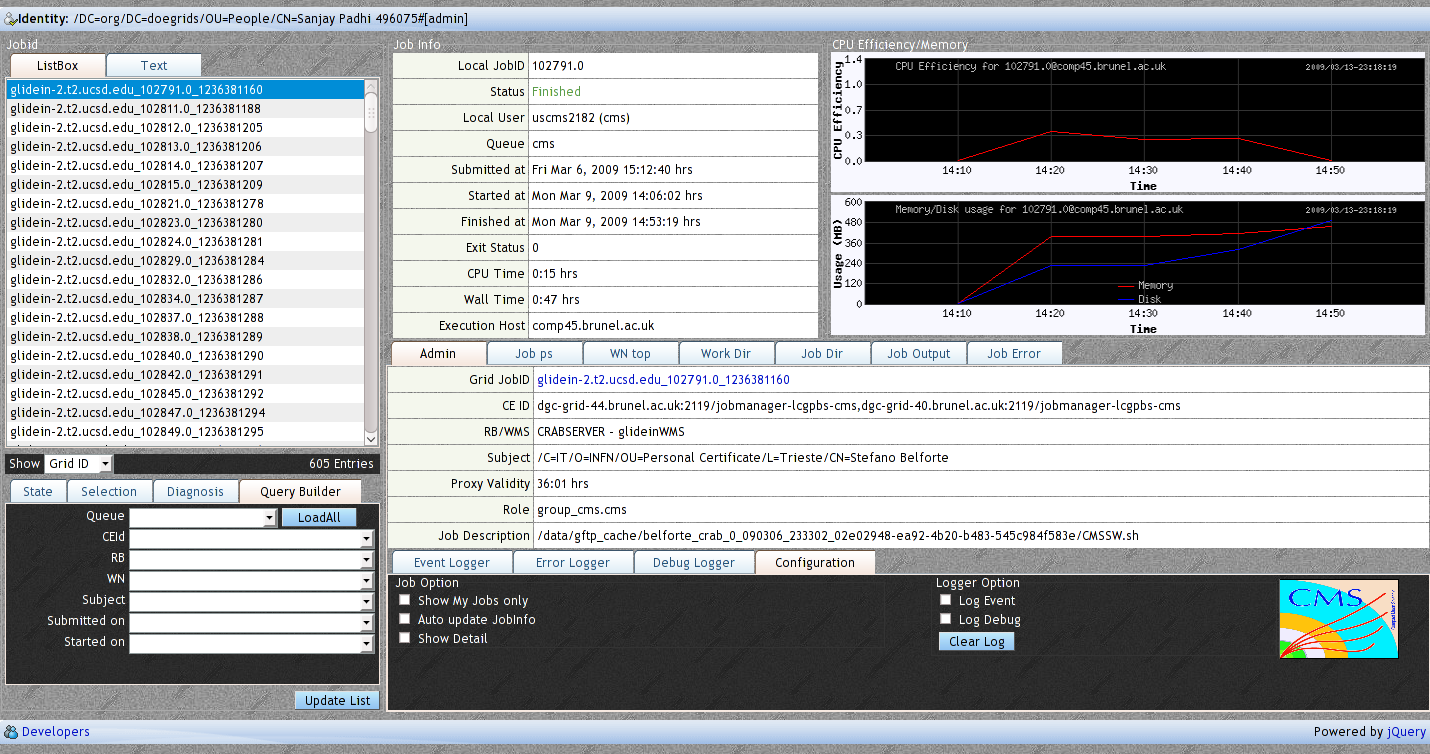
\includegraphics[scale=0.4]{jobMon.png}
\end{center}
\caption{Web-based user job monitoring in quasi-real time}
\label{fig:jobMon}
\end{figure}
The glideinWMS consists of two sets of jobs: pilots (glide-ins) and the user jobs. The
pilot jobs, as well as the submission rates, are monitored using the information from the \emph{collector},
\emph{submitter} and the retrieved output after the termination of the glide-ins via Condor-G.
Fig.~\ref{fig:glideinT1stat} for example, shows the pilot statistics and its client usage.

However, it is essential both for the end-users and the glideinWMS administrator to have 
a secure and transparent access to the real-time job monitoring. This is achieved using
``detailed job monitoring'' discussed in detail at \cite{bib:cms_jobmon}. The framework enables users to track jobs 
in substantial detail in quasi-real time as shown in Fig.~\ref{fig:jobMon}. The monitoring system aims to 
achieve the following goals:
\begin {itemize}
\item 
For the end users to be able to track jobs using job ID and get 
\subitem
- the summary information, process list
\subitem
- CPU, memory and disk usage as a function of time
\subitem
- job and working directory listing
\subitem
- access to the log files (e.g stdout, stderr)
\subitem
- status of the node that runs a job as well as site CE
\subitem
- submission/start time
\item
For the administrators in real time to
\subitem
 - track jobs using local job ID
\subitem
- find faulty worker nodes
\subitem
- for local queues/users
\subitem
- mis-behaving jobs (0 load, expiring proxies, etc.), in order to spot the problems immediately.
\end{itemize}
The framework sensors uses the information from the glide-in \emph{collector} and \emph{schedular} to
update the data at a regular interval to a MySql Database. The database serves the monitoring
information to the clients. The interface provides info regarding the state, selection, as well as 
diagnosis such as CPU, load, Memory usage in quasi-real time in order for the users to track down 
mis-behaved jobs. The database also stores summary information for the already completed jobs for archival 
purposes. The monitoring system is currently under active development and promises to provide for the first 
time access to the logs in real time of the currently running jobs at remote sites, using 
pseudo-interactive monitoring \cite{bib:pseudo_mon}.
%%%%%%%%%%%%%%%%%%%%%%%%%%%%%%%%%%%%%%%%%%%
\section{Experience using next generation CREAM CE}
%%%%%%%%%%%%%%%%%%%%%%%%%%%%%%%%%%%%%%%%%%%
\begin{figure}
\begin{center}
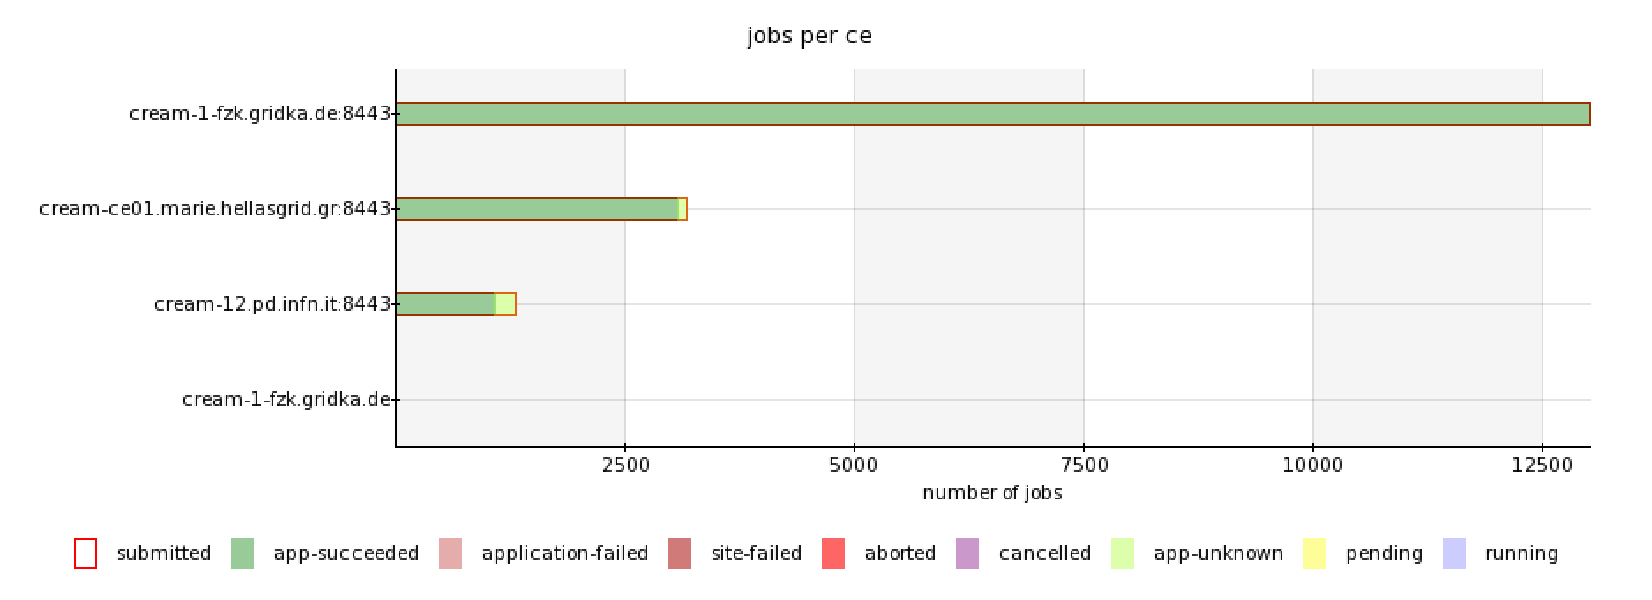
\includegraphics[scale=0.45]{cms_cream}
\end{center}
\caption{Number of resources used during the CMS tests of the CREAM CE.}
\label{fig:cms_cream}
\end{figure}
The Computing Resource Execution And Management (CREAM) is a next generation lightweight service 
for job management operation at the CE level. Recent developments to Condor-G have focused on adding 
support for CREAM. This is accomplished for the first time by using CREAM specific GHAPs. It consists 
of various algorithms responsible for communication with the CE at different stages of job submission
procedure. The responses from the CE are sent back to the Condor Gridmanager, which then updates 
the state of the jobs based on the provided info. The log retrieval is managed by Condor itself.

More than 10k jobs are submitted to the resources available via the CREAM CE using the ``modified'' Condor-G as 
shown in Fig.~\ref{fig:cms_cream}. We observed a 25\% failure rate, mostly due to proxy renewal/delegation. 
This problem is under investigation with the CREAM developers. Overall based on the successful jobs
the approach towards using CREAM as a future computing element is found to be extremely promising.
%%%%%%%%%%%%%%%%%%%%%%%%%%%%%%%%%%%%%%%%%%%
\section{Conclusion}
%%%%%%%%%%%%%%%%%%%%%%%%%%%%%%%%%%%%%%%%%%%
GlideinWMS has been widely used in CMS for central data reprocessing, skimming at the Tier-1 centers, as well
as user analysis using either CRAB client or server. It provides a homogeneous pool of resources over
heterogeneous grid environment. CRAB-based user analysis efficiency benefits significantly from the late
binding approach. Detailed job monitoring tools associated with the WMS, provides tools for the users to access 
jobs interactively for debugging. This is expected to enhance the user participation into the debugging 
infrastructure of the grid. Interface to the next generation CREAM CE has been created using Condor client. 
The preliminary results shows a significant potential in this new CE for worldwide usage. 
%%%%%%%%%%%%%%%%%%%%%%%%%%%%%%%%%%%%%%%%%%%
\section*{References}
%%%%%%%%%%%%%%%%%%%%%%%%%%%%%%%%%%%%%%%%%%%
\begin{thebibliography}{15}

\bibitem{bib:scalability} 
D. Bradley et al, ``Interoperability and Scalability within glideinWMS'', CHEP 09, Prague, Czech Republic.
\bibitem{bib:cms_computing_arch} 
CMS Collaboration 2005, CMS Computing Technical Design Report, CERN-LHCC-2005-023.
\bibitem{bib:cms_phedex}
J. Rehn et al, ``PhEDEx high-throughput data transfer management system'', CHEP06, Mumbai, India.
\bibitem{bib:cms_crab}
D. Spiga, ``Automatization of User Analysis Workflow in CMS'', CHEP 09, Prague, Czech Republic.
\bibitem{bib:cms_glite}
A. Fanfani, ``Commissioning Distributed Analysis at the CMS Tier-2 Centers'', CHEP 09, Prague, Czech Republic.
\bibitem{bib:cms_jobmon}
S. Sarkar, et al., ``A Grid Job Monitoring System'', CHEP 09, Prague, Czech Republic.
\bibitem{bib:pseudo_mon}
D. Bradley, M. Livny and I. Sfiligoi, ``Pseudo-interactive monitoring in distributed computing'', CHEP 09, Prague, Czech Republic.
\end{thebibliography}
\end{document}
